\documentclass[a4paper, 12pt]{article}
\usepackage[a4paper,margin=1.5cm]{geometry}
\usepackage[utf8]{inputenc}
\usepackage[T1]{fontenc}
\usepackage[polish]{babel}
\usepackage{graphicx}
\usepackage{hyperref}
\usepackage{listings}
\usepackage{xcolor}
\usepackage{float}

\title{Dokumentacja aplikacji Unordered}
\author{Adam Dybcio\endline
        Łukasz Czapski\endline
        Igor Ciżewski\endline
        Denis Jabłoński\endline
        Mateusz Sztankiewicz}
\date{\today}

\begin{document}

\maketitle
\newpage
\tableofcontents
\newpage

\section{Wprowadzenie}
\subsection{Cel dokumentu}
Dokumentacja ma na celu przedstawienie architektury oraz funkcjonalności aplikacji Unordered.
Zawiera również informacje o integracji z OpenAI oraz wdrożeniu aplikacji.

\subsection{Wyjaśnienie pojęć}

\begin{description}
    \item[\textbf{Box}] W kontekście aplikacji Unordered, \emph{box} to spersonalizowany zestaw prezentowy, generowany automatycznie na podstawie profilu osoby obdarowywanej, okazji, budżetu lub wyboru losowego. Box zawiera propozycje konkretnych produktów, które razem tworzą gotowy do wręczenia prezent. Każdy box jest unikalny i dopasowany do wybranych przez użytkownika kryteriów.

    \item[\textbf{AI}] Sztuczna inteligencja, w kontekście aplikacji Unordered odnosi się do wykorzystania modeli językowych OpenAI (np. o4-mini) do generowania spersonalizowanych propozycji prezentów na podstawie kryteriów podanych przez użytkownika.
\end{description}

\newpage
\subsection{Opis aplikacji}
Unordered to nowoczesna aplikacja mobilna, która pomaga użytkownikom w szybkim i trafnym wyborze prezentów na różne okazje,
takie jak urodziny, rocznice czy święta. Głównym celem aplikacji jest automatyzacja procesu doboru prezentów oraz
przypominanie o ważnych datach, eliminując problem braku pomysłów, czasu czy zapominania o okazjach.

Użytkownik może tworzyć profile osób, dla których planuje prezenty, określając ich zainteresowania i preferencje.
Następnie, dzięki integracji z AI (OpenAI GPT), aplikacja generuje spersonalizowane propozycje prezentów (tzw. boxy),
dostosowane do profilu, okazji oraz budżetu. Możliwe jest także ustawienie cyklicznych boxów, które automatycznie
przypominają i generują prezenty na wybrane daty.

Unordered wyróżnia się pełną automatyzacją - od analizy profilu, przez dobór produktów z wielu platform zakupowych,
aż po przypomnienia o nadchodzących okazjach. Dzięki temu użytkownik nie musi samodzielnie przeszukiwać sklepów ani
pamiętać o terminach - aplikacja zrobi to za niego, zapewniając jednocześnie element zaskoczenia i personalizacji.

Aplikacja jest skierowana zarówno do osób prywatnych, jak i firm, które chcą zadbać o swoich pracowników
czy bliskich, oferując im wyjątkowe, dopasowane prezenty bez zbędnego wysiłku.

\begin{figure}[H]
    \centering
    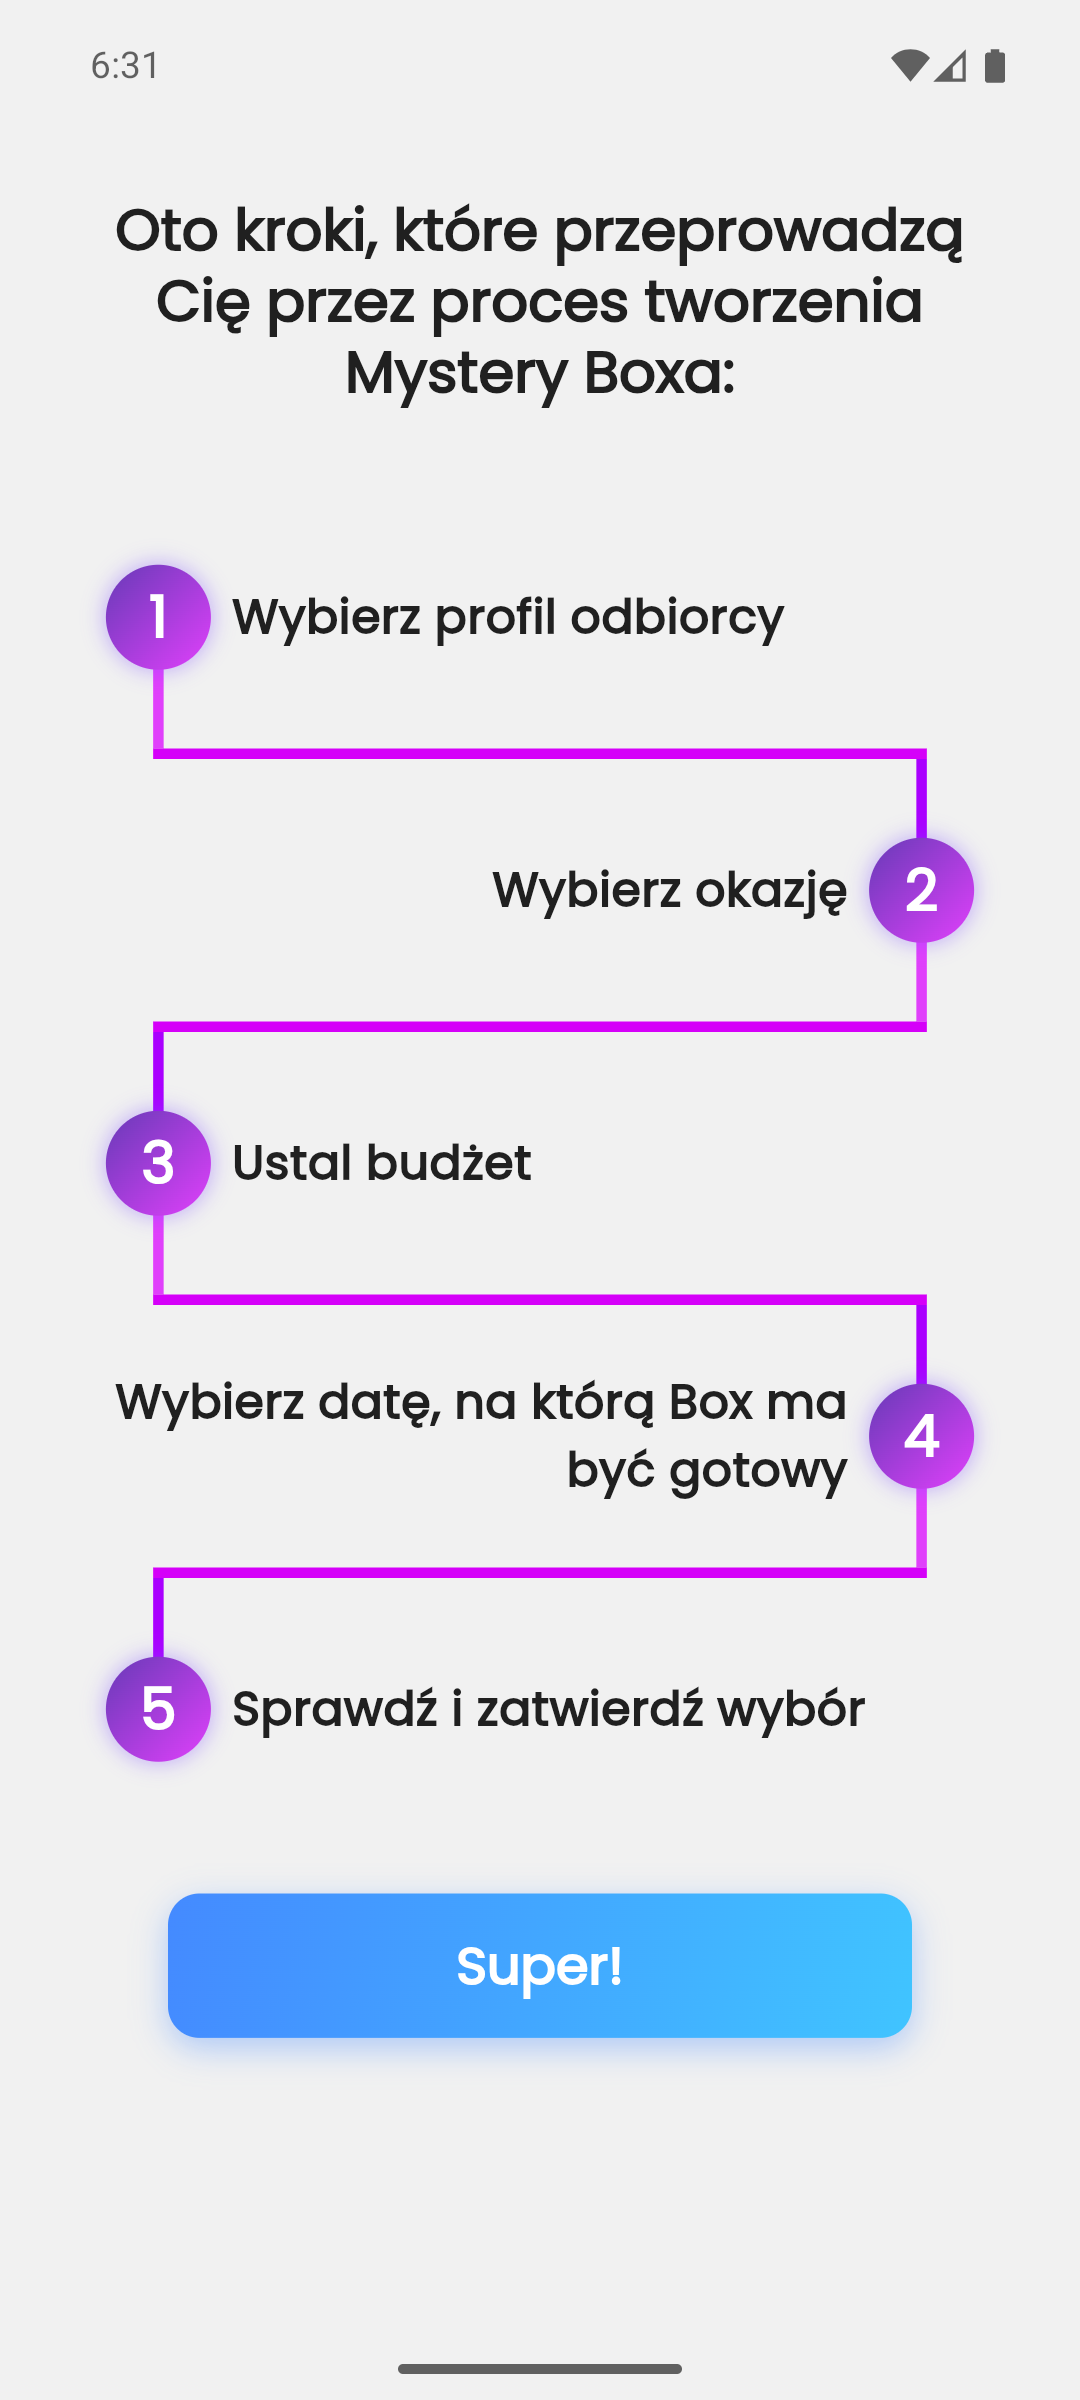
\includegraphics[width=0.3\linewidth,keepaspectratio]{images/box_desc.png}
    \caption{Opis generacji boxów dla profilu}
    \label{fig:box-desc}
\end{figure}

\newpage

\section{Architektura}
\subsection{Diagram wysokopoziomowy}
\begin{figure}[ht]
    \centering
    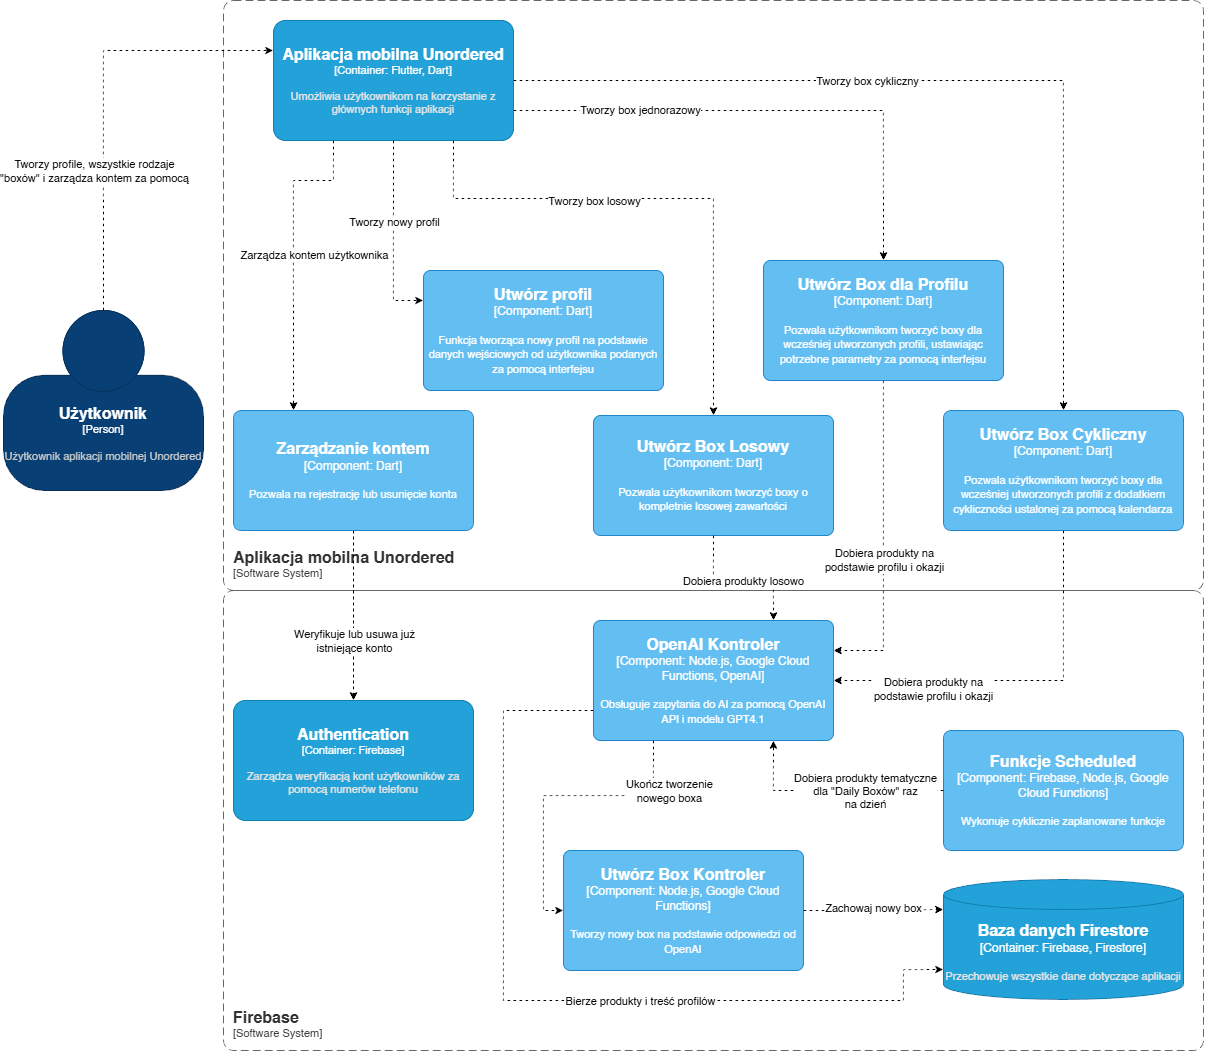
\includegraphics[height=0.745\textheight,keepaspectratio]{images/unordered.c4.png}
    \caption{Architektura systemu}
    \label{fig:architecture}
\end{figure}

\newpage

\subsection{Frontend (Flutter)}
Aplikacja mobilna Unordered została zrealizowana w technologii Flutter, co umożliwia jej uruchamianie zarówno na systemie Android, jak i iOS. Flutter pozwala na szybkie prototypowanie oraz łatwe wdrażanie zmian w interfejsie użytkownika.

\begin{itemize}
    \item \textbf{Główne pakiety:}
    \begin{itemize}
        \item \texttt{firebase\_core} -- integracja z Firebase
        \item \texttt{firebase\_auth} -- obsługa uwierzytelniania użytkowników
        \item \texttt{cloud\_functions} -- wywoływanie funkcji chmurowych backendu
        \item \texttt{cloud\_firestore} -- dostęp do bazy danych Firestore
        \item \texttt{http} -- komunikacja z zewnętrznymi API
    \end{itemize}
    \item \textbf{Główne funkcjonalności:}
    \begin{itemize}
        \item Rejestracja i logowanie użytkownika (SMS/Firebase)
        \item Tworzenie i edycja profili użytkowników
        \item Generowanie boxów prezentowych na podstawie profilu, cyklicznie lub losowo
        \item Przeglądanie historii wygenerowanych boxów
        \item Przeglądanie kalendarza z zaplanowanymi boxami
        \item Integracja z backendem (Cloud Functions, Firestore)
    \end{itemize}
\end{itemize}
\begin{figure}[H]
    \centering
    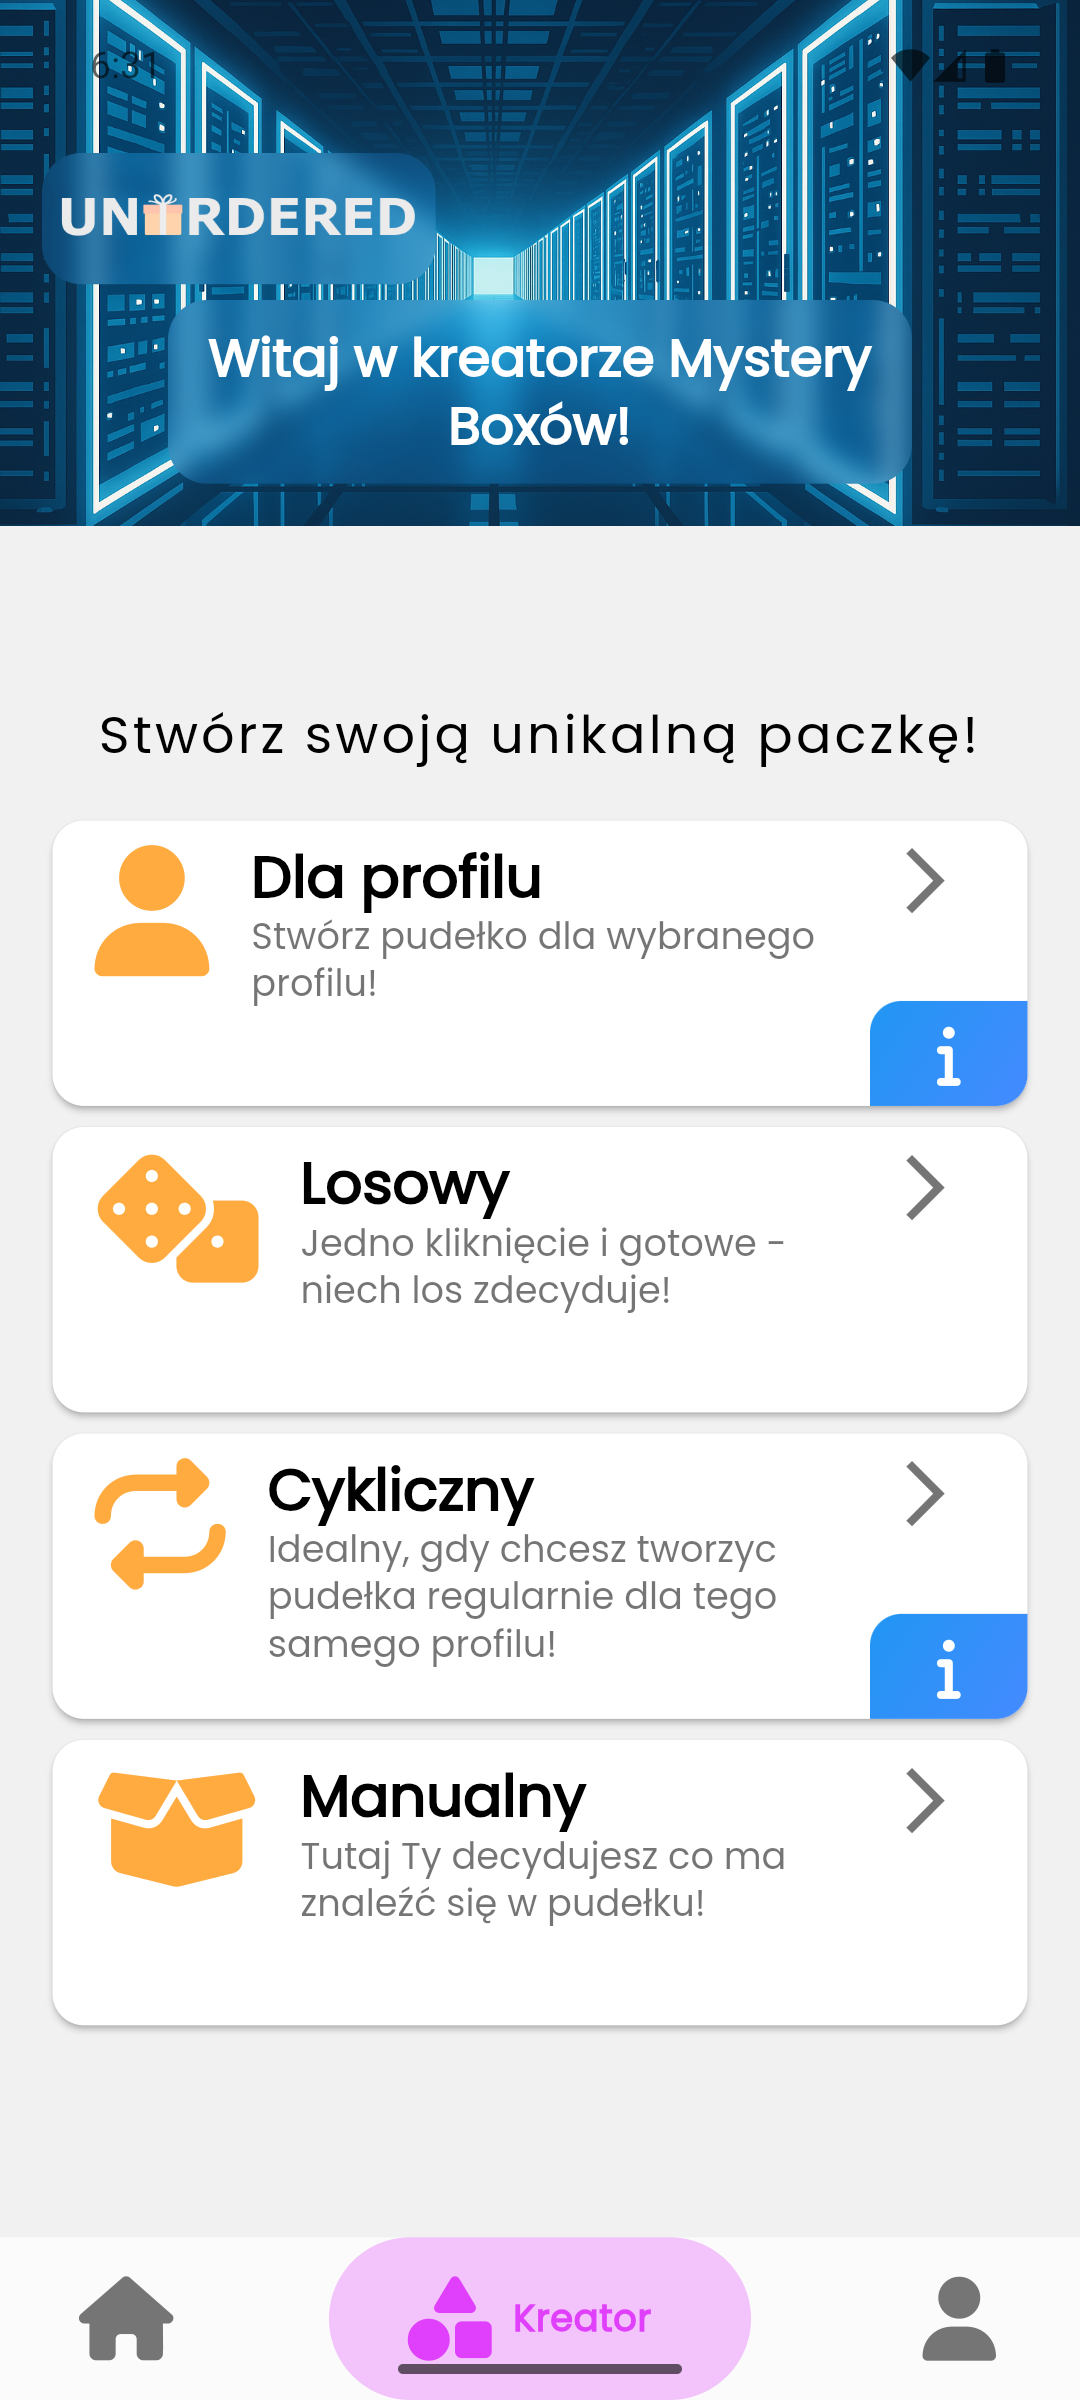
\includegraphics[width=0.3\linewidth,keepaspectratio]{images/box_creator.png}
    \caption{Kreator boxów}
    \label{fig:box-creator}
\end{figure}
\subsection{Backend (Firebase)}
\begin{itemize}
    \item \textbf{Baza danych:} Firestore -- przechowuje dane użytkowników, zapisane profile, utworzone boxy, listy produktów oraz wszelkie inne dane niezbędne do działania aplikacji.
    \item \textbf{Funkcjonalność:} Cloud Functions (Node.js) -- obsługuje główne działania backendu aplikacji, takie jak generowanie boxów, komunikacja i przetwarzanie danych z OpenAI oraz pobieranie aktualnej listy produktów.
    \item \textbf{Uwierzytelnianie:} Firebase Authentication -- pozwala użytkownikom na rejestrację i logowanie się do aplikacji za pomocą numeru telefonu, używając weryfikacji SMS.
    \item \textbf{Automatyzacja:} Cloud Functions Scheduler -- służy do cyklicznego uruchamiania funkcji, obsługuje m.in. generowanie ``Daily Boxów'' -- codziennych propozycji prezentów o losowych kategoriach.
\end{itemize}

\newpage
\section{Funkcjonalności}
%%\todo{Pokazać w screenshotach jak to działa albo to zrobić w sekcji frontend}
\subsection{Generowanie boxów}

\subsubsection{Typy generowania}
\begin{itemize}
    \item \textbf{Dla profilu} - Generacja boxów na podstawie profilu, który został wcześniej utworzony.
    Użytkownik podaje budżet oraz okazję, na którą box ma być wygenerowany.
    \item \textbf{Cykliczny} - Generacja boxów cyklicznych,
    które będą generowane co określony czas (np. co miesiąc, co rok).
    Wymagane parametry jak w przypadku boxów ``Dla profilu''.
    \item \textbf{Losowy} - Generacja losowych propozycji prezentów, bez podawania żadnych parametrów
    \item \textbf{Manualny} - aktualnie brak implementacji
\end{itemize}
\subsubsection{Profil użytkownika}
Do wygenerowania boxów typu ``Dla profilu'' lub ``Cykliczny'' wymagane jest utworzenie profilu, dla którego dobierane będą propozycje. Dane profilu to:
\begin{itemize}
    \item \textbf{Nazwa profilu} (np. ``Mama'', ``Tata'', ``Kolega'')
    \item \textbf{Opis osoby} (Preferencje, zainteresowania, itp.)
    \item \textbf{Zainteresowania} (Wybór kategorii z gotowej listy)
\end{itemize}

\newpage

\subsection{Struktura boxa}
Struktura boxów jest taka sama dla wszystkich typów generowania. Boxy są przechowywane w bazie danych Firestore i zawierają następujące dane:
\begin{itemize}
    \item \textbf{Budżet} (kwota, którą użytkownik chce przeznaczyć na prezenty)
    \item \textbf{Data wygenerowania} (data, kiedy box został wygenerowany)
    \item \textbf{Czy jest cykliczny} (wartość logiczna, czy box jest cykliczny)
    \item \textbf{Frekwencja cykliczności} (używane tylko dla boxów cyklicznych, np. co miesiąc, co rok)
    \item \textbf{Okazja} (okazja, na którą box został wygenerowany, np. urodziny, imieniny)
    \item \textbf{Planowana data} (data, na którą box został zaplanowany)
    \item \textbf{Cena} (suma cen wszystkich produktów w boxie)
    \item \textbf{Lista produktów} (produkty, które zostały wygenerowane w boxie)
\end{itemize}
\begin{figure}[H]
    \centering
    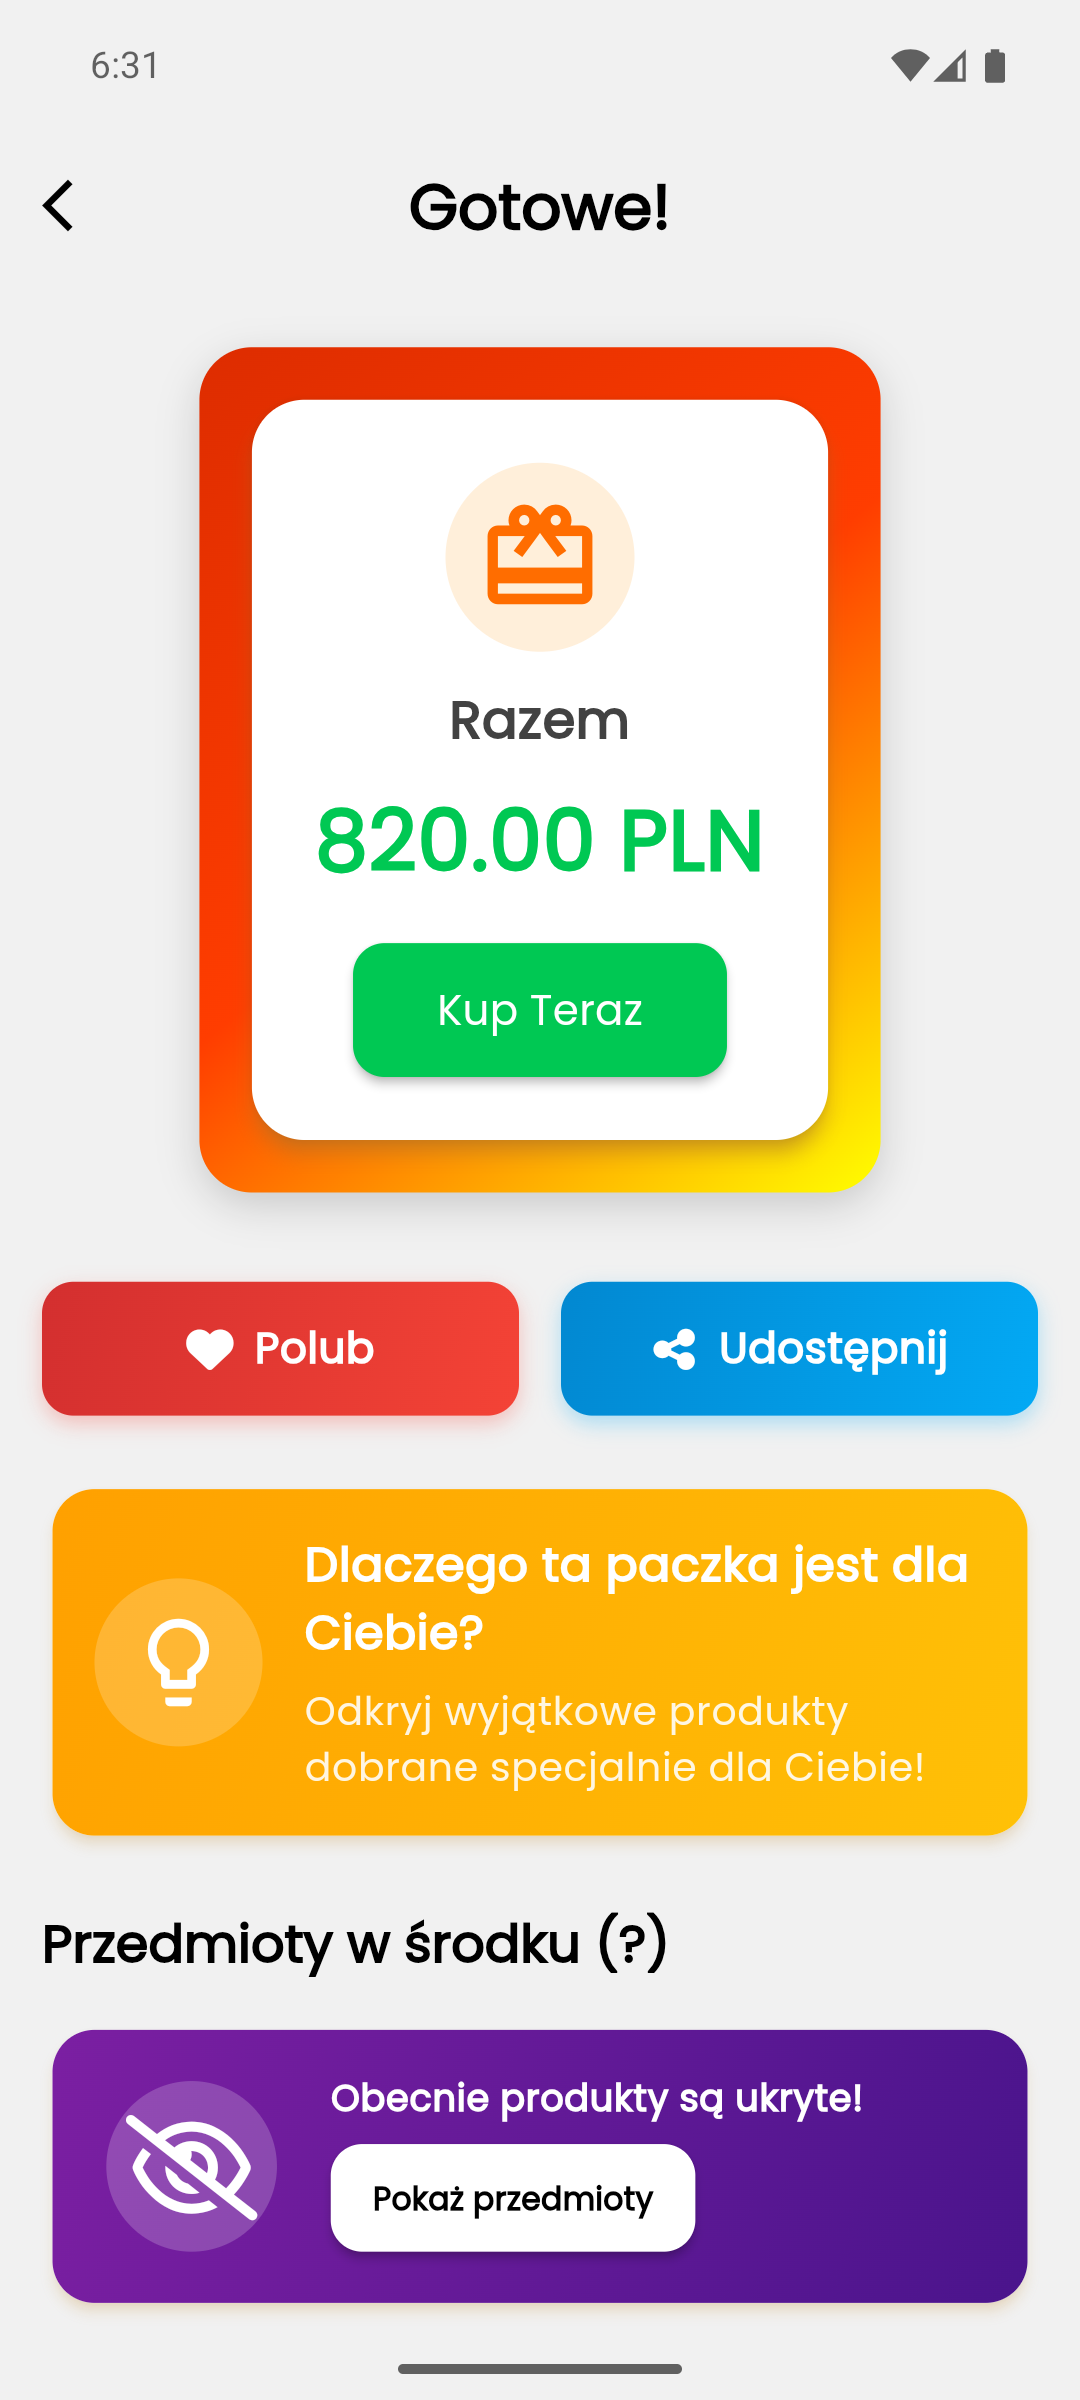
\includegraphics[width=0.3\linewidth,keepaspectratio]{images/box_summary.png}
    \caption{Widok wygenerowanego boxa}
    \label{fig:box-summary}
\end{figure}
\newpage
\section{Integracja z OpenAI}
\subsection{Opis API}
Wybranym do generacji modelem jest \textbf{OpenAI o4-mini}.
Wybór modelu jest uzasadniony
jego działaniem w trybie ``reasoning'' który pozwala na generacje biorącą pod
uwagę wszystkie parametry podane przez użytkownika.
Jest on również tańszym wyborem, w porównaniu do modeli \textbf{GPT-4.1} oraz \textbf{OpenAI o3}.
\subsection{Prompt engineering}
Przy inżynierii promptów uwaga była skupiona na wykorzystaniu najmniejszej liczby tokenów przy zachowaniu jak najlepszej jakości odpowiedzi.
Strukturą wszystkich promptów jest:
\textbf{ZASADA}$\rightarrow$\textbf{OPIS ZASADY}
\begin{itemize}
    \item \textbf{Generowanie boxów dla profilu} - generacja boxów na podstawie profilu użytkownika.\\\\
        \textbf{ANALIZA}$\rightarrow$Uwzględnij zainteresowania, okazję (...) \\
        \textbf{RÓŻNORODNOŚĆ}$\rightarrow$Unikaj powtórzeń, (...) \\
        \textbf{BUDŻET}$\rightarrow$Nigdy nie przekraczaj budżetu!(...) \\
        \textbf{ODPOWIEDŹ}$\rightarrow$Zwróć TYLKO JSON array (...) \\
    \item \textbf{Generowanie ``Daily Boxów''} - generacja boxów o różnych tematach, raz dziennie.\\\\
        \textbf{DOBÓR}$\rightarrow$Uwzględnij temat, unikaj innych kategorii. (...) \\
        \textbf{RÓŻNORODNOŚĆ}$\rightarrow$Unikaj powtórzeń,  (...) \\
        \textbf{BUDŻET}$\rightarrow$Nigdy nie przekraczaj budżetu!  (...) \\
        \textbf{ODPOWIEDŹ}$\rightarrow$Zwróć TYLKO JSON array  (...) \\
    \item \textbf{Generowanie losowych boxów} - generacja boxów bez podawania żadnych parametrów.\\\\
        \textbf{LOSOWOŚĆ}$\rightarrow$Wybierz losowe przedmioty (...) \\
        \textbf{RÓŻNORODNOŚĆ}$\rightarrow$Dobieraj różne kategorie. \\
        \textbf{BUDŻET}$\rightarrow$Utrzymaj realistyczny budżet.\\
        \textbf{ODPOWIEDŹ}$\rightarrow$Zwróć TYLKO JSON array (...) \\
\end{itemize}
\subsection{Przetwarzanie odpowiedzi}
Formatem zwróconej odpowiedzi jest JSON array, który zawiera listę samych ID produktów,
aby zminimalizować liczbę tokenów. Następnie ID są sprawdzane oraz przetwarzane przez backend.

\section{Wdrożenie}
\subsection{Konfiguracja Firebase}
Aby wdrożyć funkcje chmurowe (Cloud Functions) za pomocą Firebase,
należy użyć narzędzia \texttt{firebase} dostępnego przez npm,
oraz zainicjować projekt i wdrożyć funkcję do projektu Firebase.
Po wdrożeniu należy upewnić się, że adresy (linki) do nowych funkcji są zgodne
zarówno w kodzie backendu (Cloud Functions), jak i w wywołaniach po stronie frontendu Flutter.
Spójność nazw i endpointów jest kluczowa dla poprawnej komunikacji między aplikacją a backendem.

\newpage
\section{Podsumowanie i dalszy rozwój}

Aplikacja wyróżnia się na tle konkurencji pełną automatyzacją,
możliwą integracją z platformami zakupowymi oraz możliwością personalizacji prezentów na podstawie
profilu obdarowywanej osoby. Dzięki temu użytkownik zyskuje pewność, że prezent będzie trafiony,
a cały proces przebiegnie sprawnie i bez zbędnego wysiłku.

\subsection{Znane ograniczenia}
\begin{itemize}
    \item Ograniczenia i limity związane z wykorzystaniem API OpenAI (np. limity tokenów, koszty).
    \item Limity Firebase dotyczące liczby operacji, przechowywania danych i autoryzacji.
    \item Dostępność produktów zależna od integracji z zewnętrznymi platformami zakupowymi.
    \item Brak pełnej automatyzacji zamówień fizycznych (na obecnym etapie aplikacja generuje propozycje, nie realizuje zamówień).
\end{itemize}

\subsection{Roadmap}
Wśród planowanych kierunków rozwoju aplikacji znajdują się:
\begin{itemize}
    \item Integracja z dodatkowymi platformami zakupowymi, co pozwoli na jeszcze szerszy wybór produktów.
    \item Współpraca z markami i sklepami -- możliwość tworzenia dedykowanych boxów z konkretnych sklepów lub marek.
    \item System subskrypcji -- użytkownik mógłby otrzymywać cykliczne, personalizowane boxy za miesięczną lub roczną opłatą.
    \item Rozbudowa funkcji kalendarza i przypomnień, w tym integracja z kalendarzem Google lub Outlook.
    \item Współpraca z influencerami i działania marketingowe skierowane do młodych, zabieganych osób.
    \item Usprawnienie procesu zamawiania -- możliwość bezpośredniego zamówienia produktów z poziomu aplikacji.
    \item Rozszerzenie funkcjonalności AI o jeszcze lepsze dopasowanie prezentów do profilu użytkownika.
\end{itemize}

Unordered jest projektem otwartym na dalszy rozwój i nowe pomysły,
a jego architektura pozwala na łatwe wdrażanie kolejnych funkcjonalności
w odpowiedzi na potrzeby użytkowników i rynku.

\begin{thebibliography}{9}
\bibitem{flutter}
Flutter documentation, \url{https://flutter.dev/docs}

\bibitem{firebase}
Firebase documentation, \url{https://firebase.google.com/docs}

\bibitem{openai}
OpenAI API reference, \url{https://platform.openai.com/docs/api-reference}
\end{thebibliography}

\end{document}